\chapter{Population Proportion Statistics}

Let's say that you are trying to get a candidate elected.  The candidate asks you, "What proportion of the voting population is going to vote for me?"  
So, you go out and ask a random sample of 12 voters.  11 say that they are going to vote for your candidate.  What can you tell the candidate?

\section{Sample Probabilities from Population Proportion}

To address these sorts of questions (and there are a lot of them),  we start with the opposite question:  If we knew what the proportion was in the 
entire population,  what sort of results should we expect in a random sample of just 12?

For example,  let's say that 62\% of the entire population plans to vote for your candidate. You ask 12 people, "Will you vote for my candidate?"  How many will say "Yes"?  You don't know --- it depends
on the sample. For example,  there is some chance that you will just happen to choose all 12 from the 48\% of the population that does not plan to vote for your candidate.

We can compute the probability of each outcome using the binomial distribution. Let $r$ be the probability that a random person will say, "I plan to vote for your candidate."  Let $n$ be the number of people 
you ask.  The probability that exactly $k$ people will say, "I plan to vote for your candidate"  is given by:

$$p(k) =  \binom{n}{k}r^k(1-r)^{n-k}$$

Note that even though most people support your candidate,  there is some chance that no one you ask will say that they will vote for your candidate. 

Using $r=0.62$,  we can compute the probability of each outcome:


\begin{tabular}{r | r}
$k$  & $p(k)$ \\
\hline
0 & 0.000009 \\
1 & 0.000177 \\
2 & 0.001593 \\
3 & 0.008663 \\
4 & 0.031801 \\
5 & 0.083017 \\
6 & 0.158024 \\
7 & 0.220996 \\
8 & 0.225358 \\
9 & 0.163418 \\
10 & 0.079989 \\
11 & 0.023729 
\end{tabular}

Looking at this,  the most likely outcome is that 8 people will say "Yes."  However, although it is the most like,  there is still less than a 1 in 4 chance of that outcome. It is very unlikely that less than 2 people will say "Yes."  
Here is a bar chart of the data

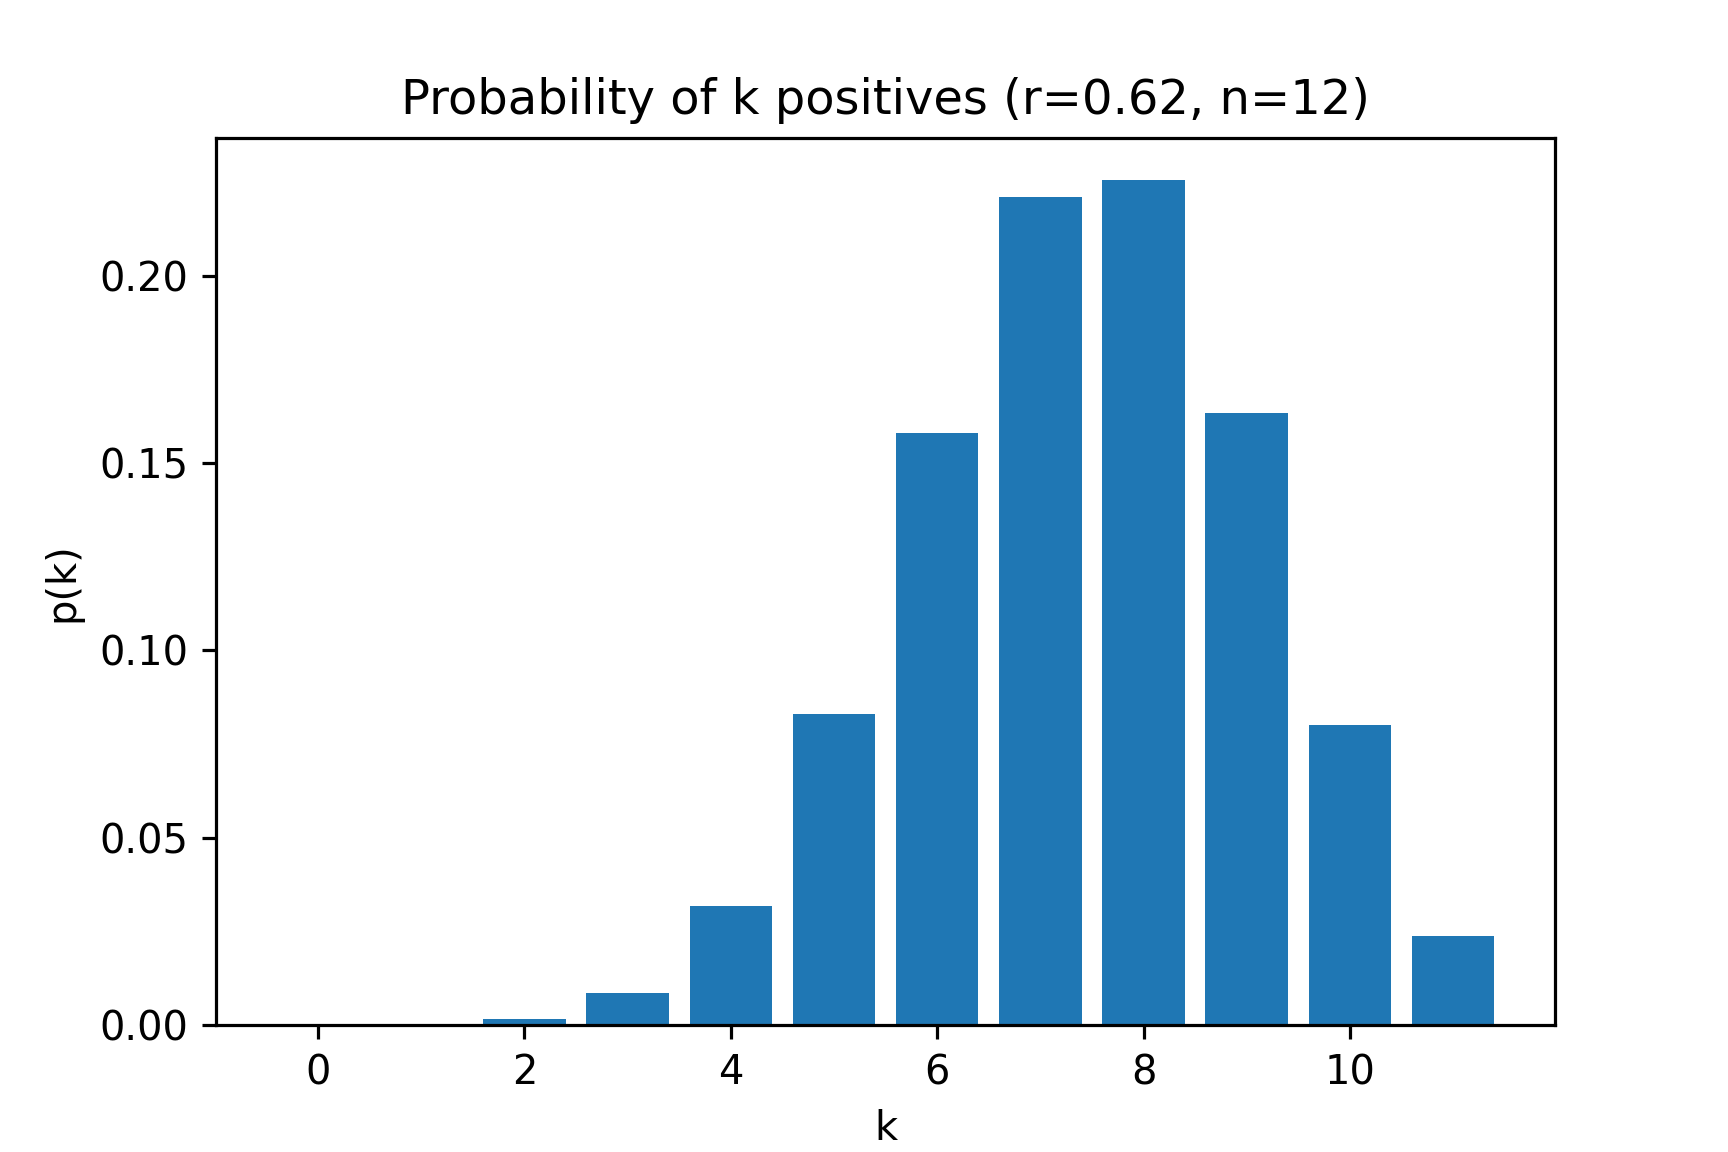
\includegraphics[width=0.8\textwidth]{binomial_dist.png}

In this section,  we knew the proportion of the population ($p$) and used that to find the probability of each possible number of positives in a random sample ($k$).  
Now, we are going to go the other way:  You know $k$, and you are finding the probability of possible values of $p$.


\section{Population Proportion from Sample}

You ask 12 people if they will vote for your candidate.  9 say "Yes."

Next, you do a thought experiment:  "If only 10\% of the population were going to vote for my candidate,  what is the probability that I would see this outcome?"

$p(9) =  \binom{n}{k}r^k(1-r)^{n-k} =  \binom{12}{9}(0.1)^9 (0.9)^{12-9} = 0.00000016$

This outcome would be quite unusual. What if 70\% of the population were going to vote for your candidate?  What is the probability that you would see this outcome?

$p(9) =  \binom{n}{k}r^k(1-r)^{n-k} =  \binom{12}{9}(0.7)^9 (0.3)^{12-9} \approx 0.2397$

In this case, the observed outcome would be a lot less unusual.

So, you decide to plot out the likelihood of this outcome for every possible value of $r$:

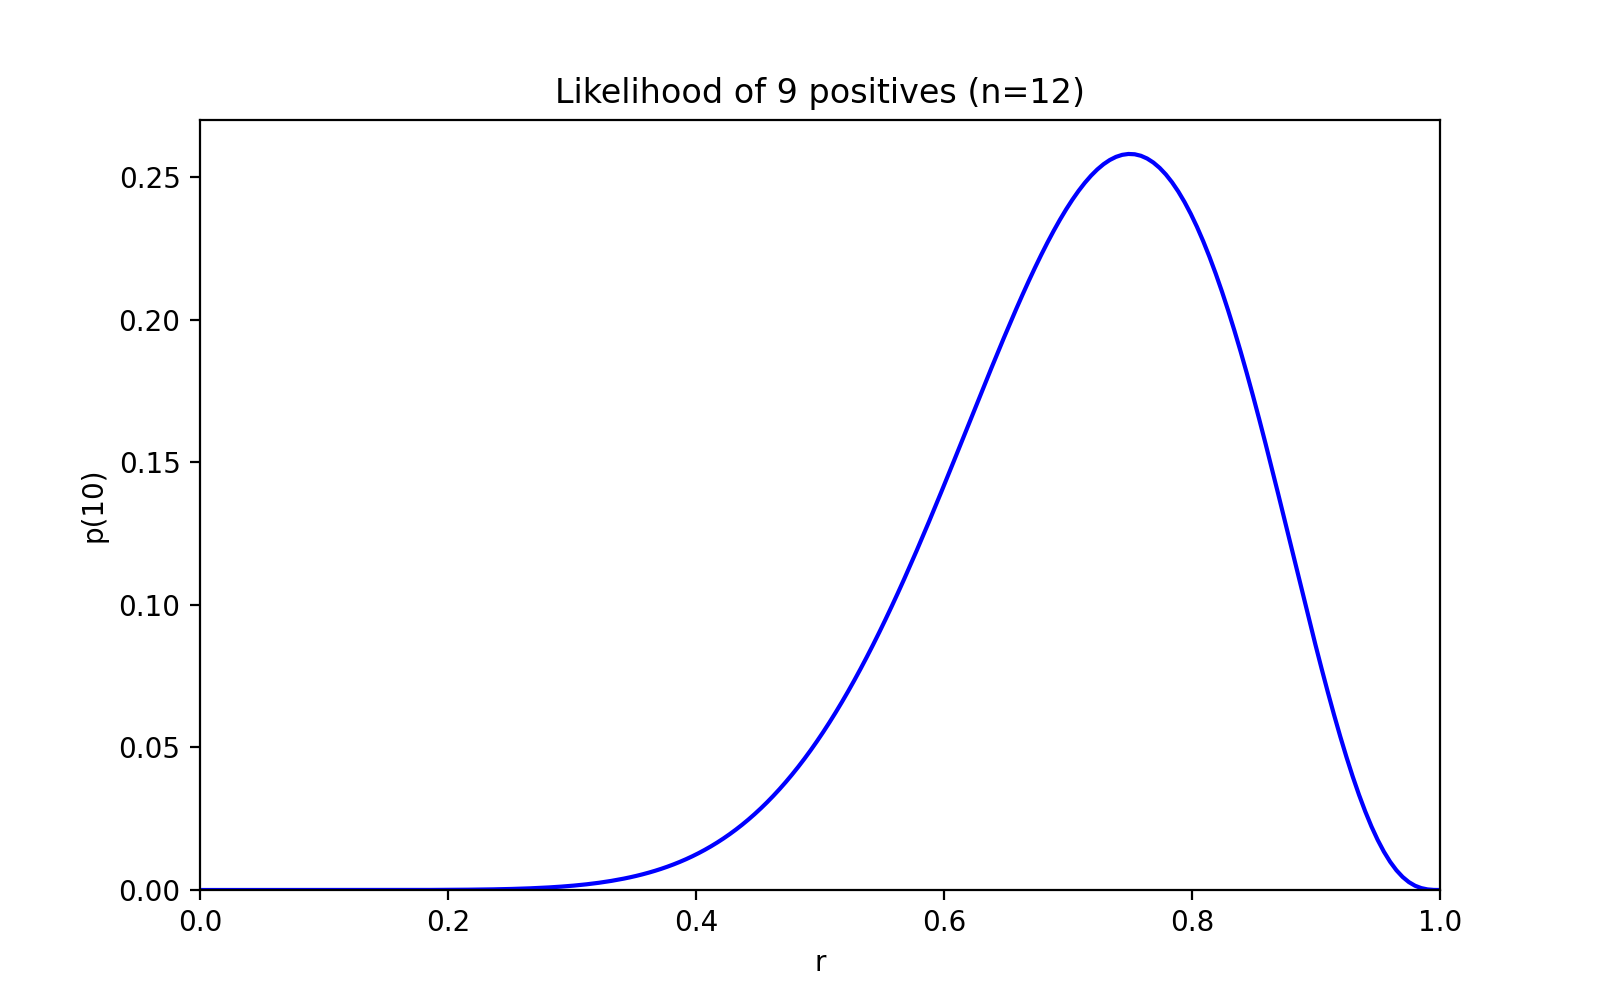
\includegraphics[width=0.8\textwidth]{likelihood.png}

This looks very similar to a probability distribution, but \emph{it is not}.  The area under the curve does not integrate to 1.0 --- it is significantly less. This is a called a \newterm{likelihood}.

However,  it still tells us something, right?  The maximum likelihood estimator is $9/12 = 0.75$.

\section{From Likelihood to Probability Density Function}

How can we make this likelihood into a probability density function?  We use Bayes' Law for continuous probability:

$$p(r|k)  = \frac{p(k | r) p(r)}{\int_{r = 0}^{1} p(k | r) p(r) dr}$$

In other words, given that we had $k$ positive responses,  what is the probability that the proportion of the population that will vote for your candidate is $r$?   The numerator of the fraction is the likelihood scaled up or down by our prior belief about the value of $r$.    What is the denominator of the fraction?  For this to be a probability distribution,  we need it to integrate to 1.  This is taken care of by the denominator.

Let's say we have no prior belief about the value of $r$.   That is, $p(r)$ is the continuous uniform distribution between 0 and 1; thus, $p(r) = 1$ for all possible values of $r$.  Our formula becomes:

$$p(r|k)  = \frac{p(k | r)}{\int_{r = 0}^{1} p(k | r) dr}$$

That is the likelihood scaled up so that it integrates to 1.  If we plot this, we get:

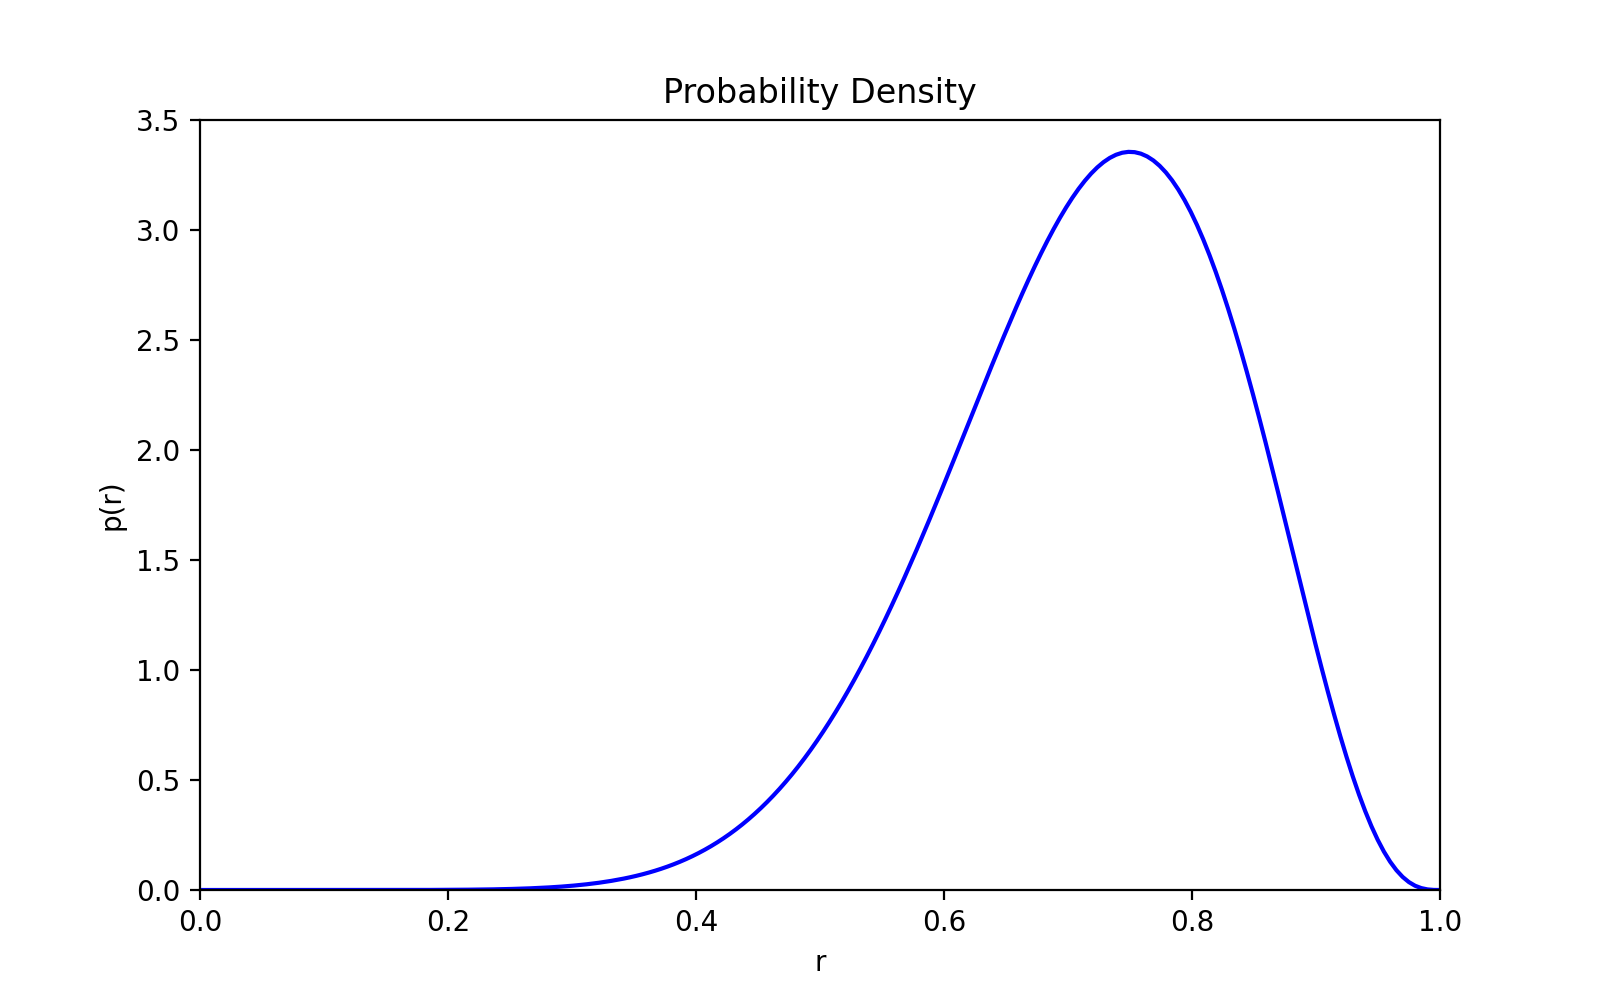
\includegraphics[width=0.8\textwidth]{bayes.png}

Here, then, is your report to your candidate: "I asked 12 voters if they were going to vote for you.  9 said yes.  Using a uniform prior,  here is what I believe about your support in the general 
population."  You also include this graph.

What happens to this graph if you ask 120 voters and 90 say yes?

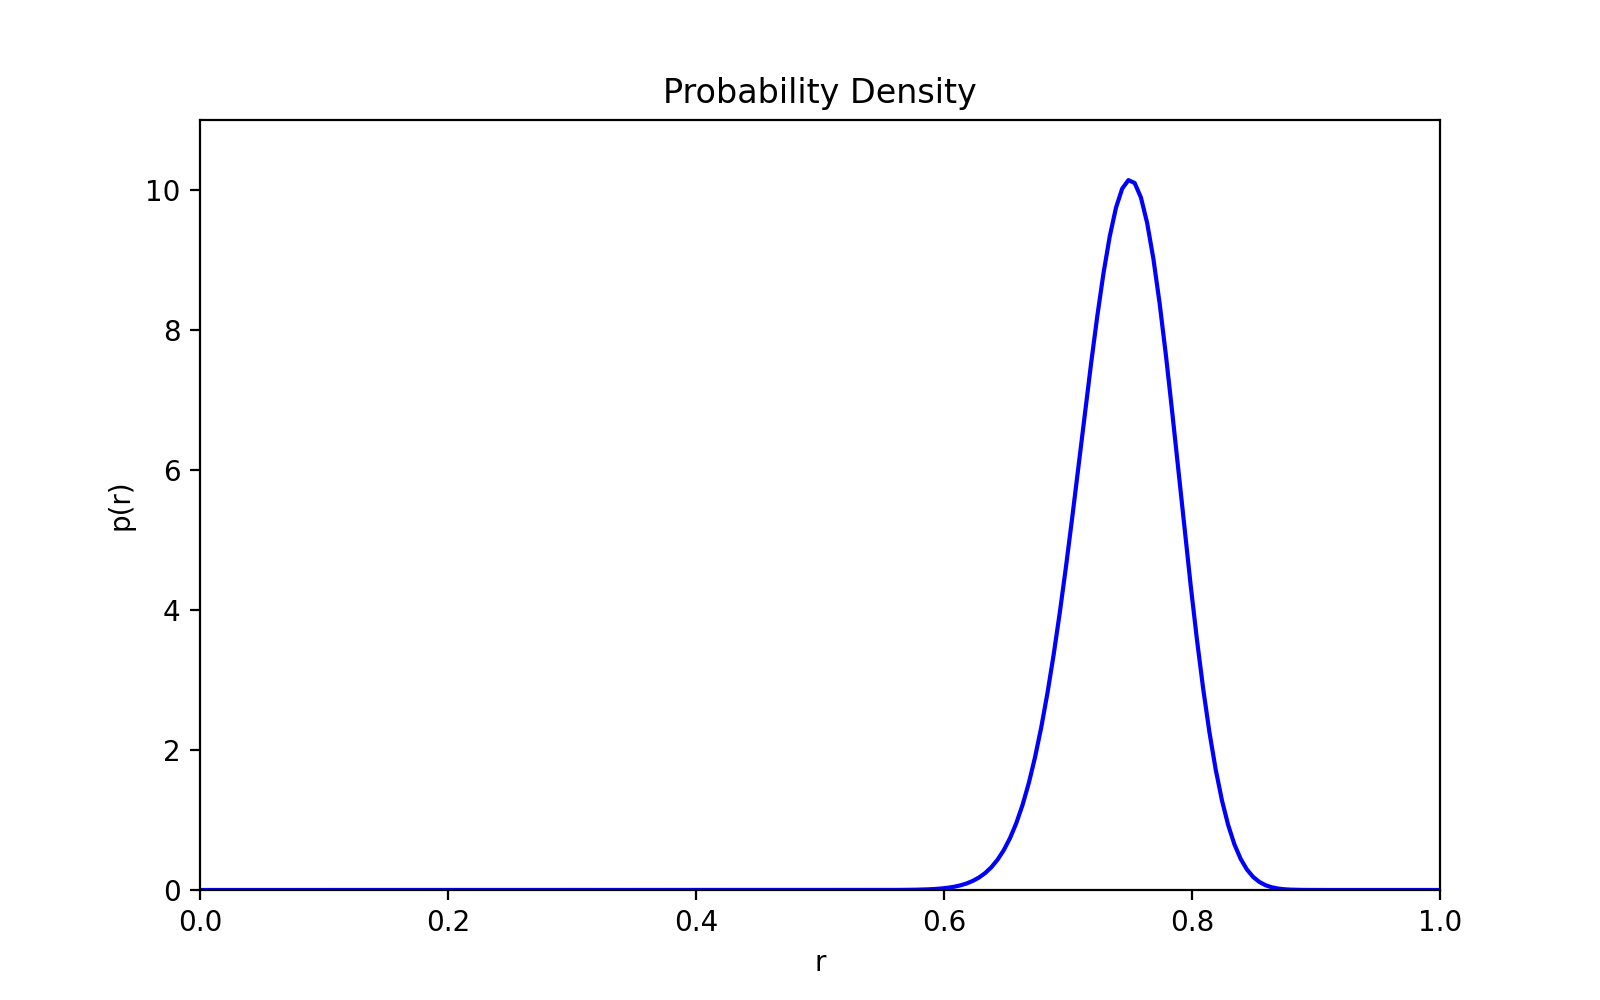
\includegraphics[width=0.8\textwidth]{bayes_tight.png}

The MLE (0.75) is the same,  but because of the much larger sample size,   you are more confident when you say "It is probably close to 75\%."

\section{Beta Distribution}

This probability distribution that you discovered is actually pretty common.  It is known as the \newterm{beta distribution}.   

The beta distribution has two parameters $a$ and $b$ that determine its shape.  If you get $k$ positives out of $n$,  then use $a = k +1$ and $b = n - k + 1$.

When you make your report to your candidate,  they will look at your probability distribution with quiet awe and ask "Based on your sample of 12 people, what is the probability that at least 50\% of the population will vote for me?"  So,  you'd fill in the region and say, "This area represents that probability."

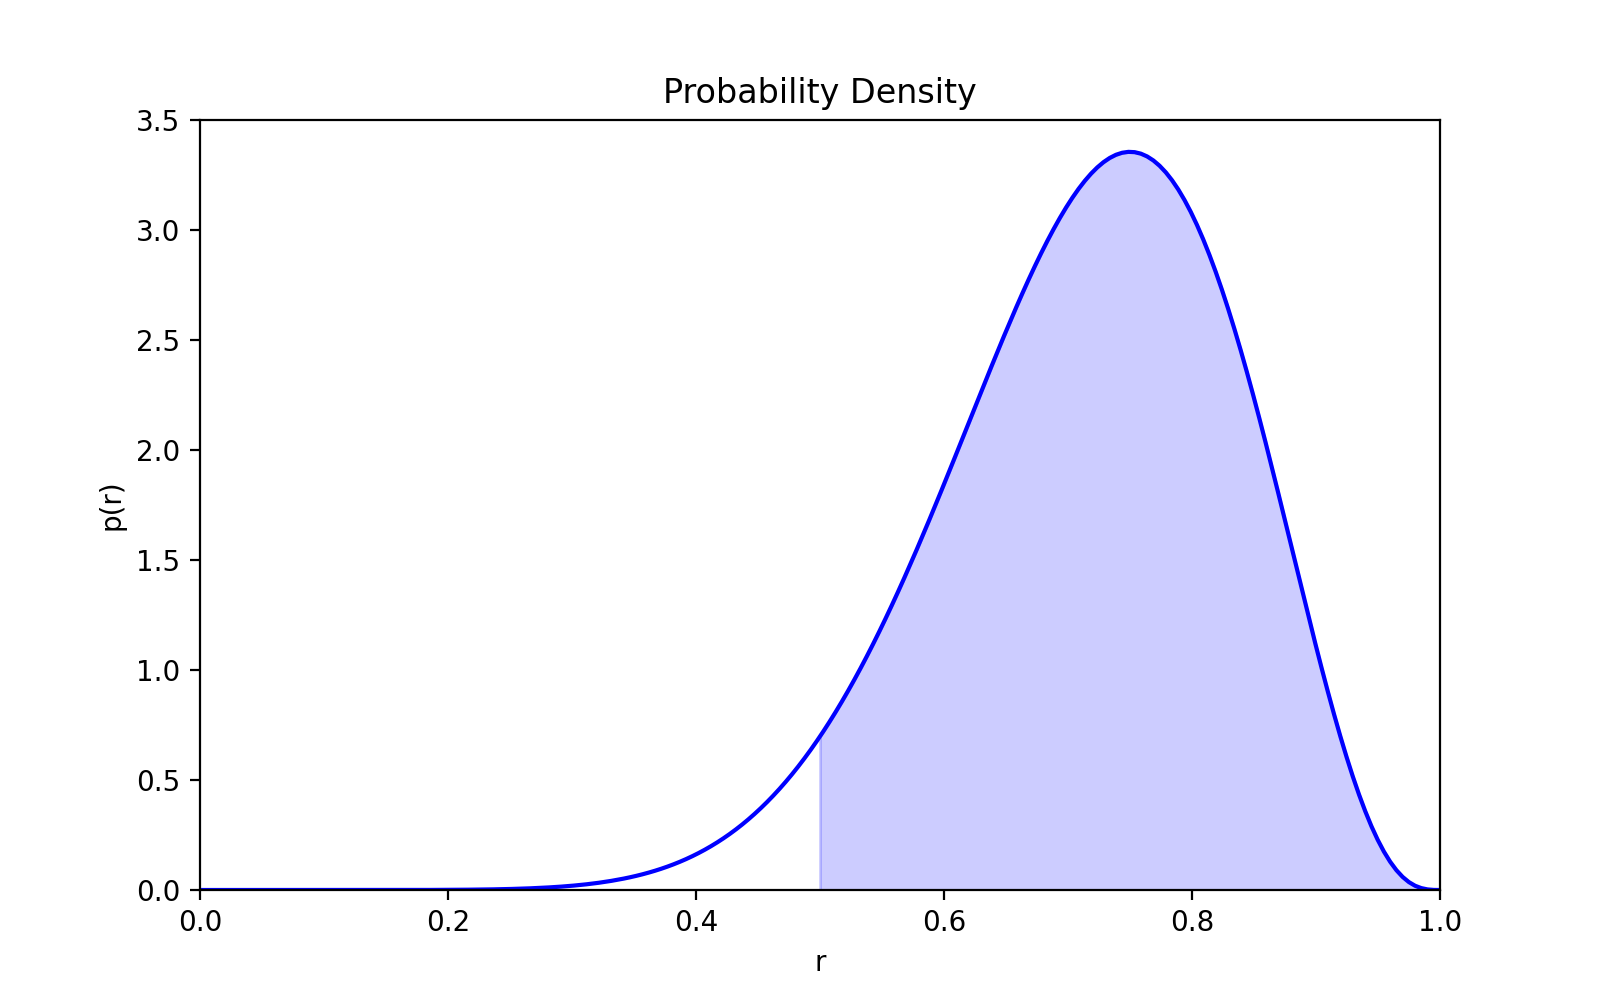
\includegraphics[width=0.8\textwidth]{bayes50.png}

Once again,  there will be a long silence, followed by a simple question: "Can you give me a number?"  Here is the Python code:

\begin{verbatim}
import numpy as np
from scipy.stats import beta

# Constants
K =  9
N = 12

# What is the probability r <=0.5?
p_less = beta.cdf(0.5, K +1, N - K +1)

# What is the probability r > 0.5?
p_more = 1.0 - p_less
print(f"I'm {p_more * 100.0:.2f}% sure you will win.")
\end{verbatim}

This will give you:
\begin{verbatim}
I'm 95.39% sure you will win.
\end{verbatim}






